%% Los cap'itulos inician con \chapter{T'itulo}, estos aparecen numerados y
%% se incluyen en el 'indice general.
%%
%% Recuerda que aqu'i ya puedes escribir acentos como: 'a, 'e, 'i, etc.
%% La letra n con tilde es: 'n.

\chapter{Design}
\newpage

This section is dedicated to explain the different important topics considered to develop a Measure System. It will be explained the architecture of the system considering its components, the physical components used to get information related to the measured materials, how was though the communication flow between the sensors and the database manager and why it was chosen the microcontrollers applied in the system.\\

There are other important requirements to consider for this project. One of these requirements of the system is that it should be a flexible system where the components used on it should have a low price. This point is relevant because it is necessary to choose the appropriate hardware to design the final solution.\\

Also, it will be explained why this solution is one of the best to apply to the of the client. This is an important topic to consider because to solve problems it is possible to apply distinct solutions.

\section{Architecture of the system}

In this section, it will be explained the architecture of the designed system. There is an explanation about how was though the main system. Also, it is explained why this solution is one of the best to solve the exposed problem.\\

In the following picture it is possible to see how is the architecture of the designed system.\\

\begin{figure}[H]
\begin{centering}
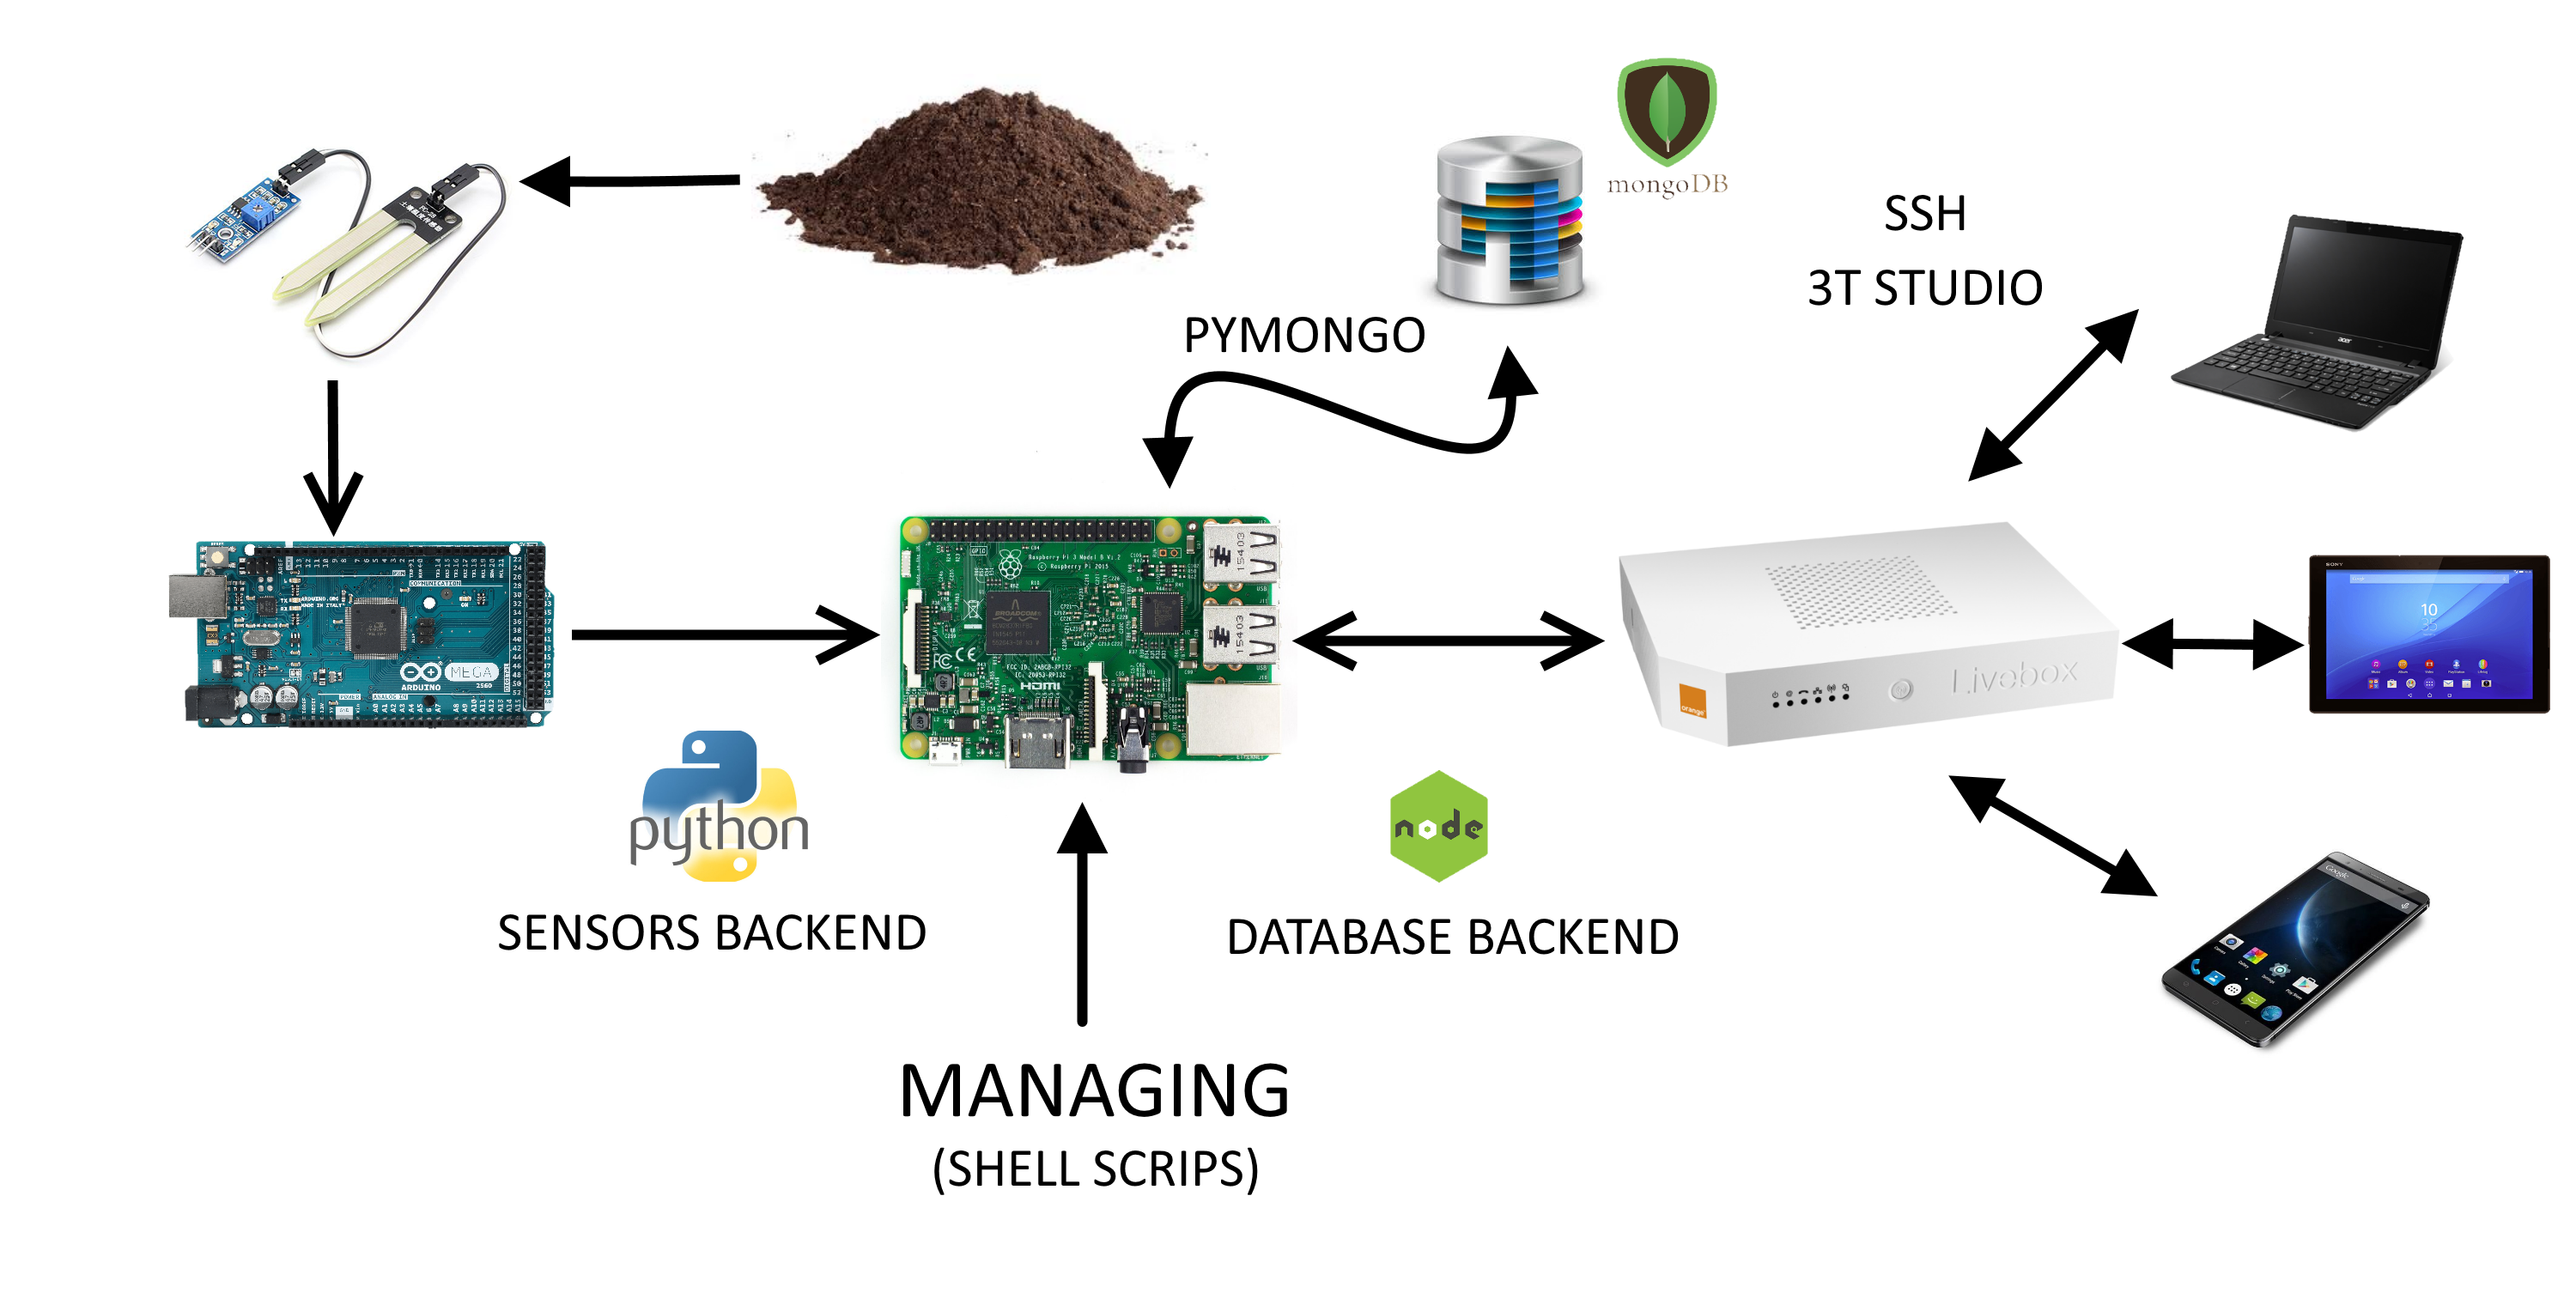
\includegraphics[scale=0.15]{IMGS/SYSTEM_SCHEMA.png}
\caption{System's architecture \label{System's architecture}}
\end{centering}
\end{figure}

The picture shows the components of the system. All the components are explained in this section.\\

All the components are interconnected, using simple communication protocols. These protocols of communication will be the following:

\begin{enumerate}

\item Serial communication. It is reliable and it avoids wireless data transfers problems between the Arduino and the Raspberry Pi \cite{what_is_raspberry_pi, raspberry_pi}. Using a serial communication will allow us to get the information without losing measures. The communication is continuous and the delay between the transfers is from five to ten seconds, avoiding problems in the communication, like flooding or missing information.

\item Ethernet communication. This communication allows us to connect the Raspberry Pi to an access point. This access point is reliable and will allow us to query the information stored in the system. We chose Ethernet to connect the Raspberry Pi to the router to avoid wireless communication problems in Raspbian \cite{raspbian} (Operative System used by the Raspberry Pi).

\item Wireless communication. We chose wireless communication to connect diverse devices to the system to query the information of the system. Those devices have to have WiFi interfaces.

\end{enumerate}

The main concept to chose all these protocols of communication is to allow a simple communication between the devices to avoid heavy tasks related to the maintain of the system. Also, all the protocols used by the system are reliable and stable.

\subsection{Data Center Processor}

In this measure system it is important to know if the information that is going to be analyzed is going to be stored or not. After talking to the client, it was considered that the system requires an amount of memory to storage the results obtained after measuring the materials.\\

With this information, it was though that it was required to use a Database Manager to store all the information coming from the sensors which are connected to the system. Also, the information measured by the system has to be obtained in a short period of time, doing this process continually. This requirement was fixed since the beginning of the project.\\

It is often applied Big Data technologies to problems where storing continuous information in a short period of time is a requirement. Big Data technologies allows us to obtain a big number of measures which allow us to analyze it after getting big amounts of information.\\

There are several technologies that allow us to apply this solution. This topic was discussed. It was important to decide which technology is applied to manage all the information measured by the sensors we had connected.\\

Another relevant requirement to consider is that the system could grow in the future. The system could have more sensors connected to measure more information. Here it was clarified that the best solution to apply to this problem was a flexible technology as Big Data technologies.\\

In the following section, it will be explained the topics related to the Data Center Processor we chose for this system.

\subsubsection{Data Center Storage}

After having several meetings to get the requirements of the system, the conclusion we reach is that the storage of the system was an important feature to consider. The \textit{Measure System} needs to store lot of information which comes from sensors which are connected to the Arduino.

Here, it was discussed if it was required to use external devices to store all the information of the sensors. We decided to use the internal storage of the system because of its fast response when it is required to query information from the database. All the information which is stored in the database has not a big size, and although the storage is continuous, the size of the database is not going to be incremented so much.\\

With this information, it is affordable to design a solution which will use a small storage device for all the information coming from the sensors. The storage of the measured information of the system is going to be done every five-ten seconds. It was defined this interval of transmission to obtain precise measures.\\

The information has to be controlled to not fill the storage used by the system. When the database will grow it is required to remove the information stored in the system. 

\subsubsection{Data Center Manager}

This part of the system is an epic for our design. The \textit{Data Center Manager} is going to manage all the information stored in the system. Also, it will manage the serial communication required to transfer the measures got from the sensors we have connected to the system.\\

This device has to allow the connectivity in case it is necessary to do tasks related to maintain. Its maintain has to be simple and easy because it will have several processes in the background running. All these processes are related to the communication of the sensors, backend \cite{backend} of the database and queries to the MongoDB database installed in the system.\\

As it was explained before, it was decided to use a Raspberry Pi 3 to control the main system. This device warrants the control of system, and also, it is a cheap solution to deploy the explained system.

\subsubsection{Data Center Controller}

The Data Center Controller of the system is related to the \textit{Data Center Manager} of the system. Both tasks are managed by the Raspberry Pi 3. This device has enough power to manage both tasks. This is the main reason we chose to use a Raspberry Pi 3, as we explained before.\\

The Data Center will be in charge of getting the information from the sensors and after getting this information, it will recognize the transmitted information storing it using the correct format for the database installed in the system.

\subsection{Sensor Controller}

To control all the sensors of the system we decided to use an \textit{Arduino Mega}. The main reason to use this device is its easy way to manage the information got from the sensors which are connected to the system. It is easy to program and easy to maintain in case it is required to do it.\\

We consider \textit{Arduino Mega} as a great controller because in case we need to upgrade the system, it will allow us to do it. It has several connections (more than the \textit{Arduino Uno}) and all these connections will allow us to connect more sensors to the system if it is required.\\

All the information transmitted by the \textit{Arduino Mega} will have a specific format to allow the Data Center Controller to recognize the information which is stored in the system. This format has to be simple and easy to be interpreted by the system.

\subsubsection{Data structures}

One of the most important requirements of the system is that the information transmitted by the sensors has to have a specific format. This format has to be defined by the developer to allow the device to recognize the information transmitted in a easy way.\\

When the information is transmitted to the controller, the controller has to recognize the parameters stored in the message. When the controller receives the information, it has to recognize from which sensor is coming the information with its current timestamp.\\

The controller is not a normal computer and the information transmitted has to be simple.

\subsubsection{Upgrades on sensors}

Since the beginning of the project, it was though that the system will have to grow in the future. The scalability of the system allows to connect more sensors to obtain more measures of soils.\\

All the upgrades done on the system have to be simple and have to avoid connection problems. We were thinking since the beginning how to do it, and the solution we designed is to connect N sensors to the system without changing parameters in the \textit{Data Controller}.\\

The \textit{Arduino Mega} is prepared to allow the connection of more sensors on the system. It is required to prepare the physical circuits to connect more sensors following the \textit{datasheet} provided in this document.\\

The normal use case of the user is to connect the sensor to the system as it is done with the others. When the sensor is connected, the system will recognize it instantly and it will start to record information from it.

\section{Information flow}

One of the most important things to consider to design the system is how is going to be the information flow. When we talk about \textit{information flow}, we refer to from which parts of the system flow the communication.\\

The way the communication is done in the system is the following:

\begin{enumerate}

\item The sensors will get the information from the substratum where they are connected.
\item The \textit{Arduino Mega} has to process the information received from the sensors and it has to define the format used to start the communication with the Raspberry Pi 3.
\item Every five seconds the \textit{Arduino Mega} will send information to the Raspberry Pi 3.
\item The Raspberry Pi has to listen continuously to the information which is coming from a serial port.
\item The Raspberry Pi has to receive the information received from the serial port, and after that, it has to parse the received information with its format.
\item When the Raspberry Pi 3 has processed the information, it has to store it with its correct format and its correct timestamp.
\item MongoDB's \cite{mongodb, pymongo} daemon has to manage the query launched by the backend of the Raspberry Pi 3 and it has to store it in the database.
\item MongoDB's daemon will wait for incoming connections where the user or the programmer will launch queries to the database. These queries could store information in the database or display the information stored in the database.
\end{enumerate}

With all these steps, the system will start to record information coming from the sensors. All the stored information will be available for the user in case the user needs to query information from the system to get results.

\subsection{Sensor information flow}

It is required to use a device which will have the possibility to get information from sensors. This device has to be connected to all the sensors and it has to have enough efficiency to manage all the information coming from the sensors of the system.\\ 

The information is received by the controller (in this design, the \textit{Arduino Mega} will do all this stuff) and it has to choose the correct format to send the information.\\

When the device has all the information of all the sensors, it has to create a message with all the information of the sensors to send it to the target device (in this case the controller which will store the information in the database).\\

The device will build a message with a specific format, and when the message is built, it will send it with the chosen format.

\subsection{Storage information flow}

When the system receives a message, it has to process it, and after that, it has to decide if the information has be stored or not.\\

The system will be listening to all the incoming messages over a serial connector. This serial connector is managed by the system. The system will control the port linked to the serial communication.\\

When the system receives a message on its serial port, it will analyze the received message and it will check its format. If the format of the message in the correct way, it will parse the message and it will send the information to the database.\\

The backend will control the communication to the database. This communication is controlled by the system, and it will send the information to the database using the supported queries of the database controller.\\

The MongoDB daemon will stay listening for all the queries launched by the system. This daemon supports concurrent connections to the database.\\

If there is a message with an incorrect format, the backend will just discard the message. This concept will allow the database to have consist and reliable information on it.

\subsection{Query information flow}

In the requirements explained in previous sections, it was decided to allow the system to store information. Also, it is defined that the user has to have access to the database created by the system to retrieve its information.\\

This concept has to be explained with the following understanding:

\begin{itemize}
\item The system has to support queries which allows the developer or the backend to store information in the database. We define this queries as internal queries used by the main system to feedback the database.
\item The system has to support external queries which will allow the users to query the information stored on it. All these queries are external to the system. The external queries do not modify the database, they display the information stored in the system.
\end{itemize}

With this information, it is clarified how is going to be the query information flow in the system. It is required to define it because all the queries related to store information in the system, are done inside the device.\\

The external queries are dedicated to show information of the database where the user will use to prepare different analysis of the data stored in the system.

\newpage
\newpage

